%Copyright (C) 2014 Sergio García Villalonga.

Per tal de poder dur a terme una avaluació de la influència de la presència d'usuaris en un precisió del sistema de localització en interiors, es necessitava un lloc que presentàs variacions de presència de persones notables. A més, tenint en compte que el sistema AirPlace es basa en la localització mitjançant una infraestructura WiFi existent, l'entorn havia de proveir una quantitat suficient de punts d'accés per dur a terme les nostres operacions.

Aquestes necessitats es veuen cobertes en edificis com els centres comercials. Les proves realitzades per aquest estudi es varen dur a terme en una secció del centre comercial Glòries, A Barcelona. La diferència horària entre l'obertura del centre als treballadors i l'obertura als clients proporciona un context idoni per realitzar proves en un entorn pràcticament buit als matins, i la proximitat de les festes de nadal a la hora de realitzar les proves han ofert un entorn molt concorregut durant l'horari comercial.

A més, l'elecció d'un centre comercial, proporciona dos tipus d'espais -passadissos i tendes- sobre els que resulta interessant classificar els resultats. El primer cas, l'entorn es caracteritza per majors espais, voltes més amples i menys presència d'obstacles entre diferents localitzacions. Per contra, a les tendes, la presència de prestatges, parets, sostres més baixos i altres obstacles, proporcionen un context en el que, a priori, la precisió es pot veure minvada, tant en el cas de absència com en el de presència d'usuaris en l'entorn.

La realització de les proves dins un centre comercial i estudiar els resultats dels dos tipus de localitzacions pot permetre, a més d'afrontar possibles millores de la manera més adequada en cada situació, donar un enfocament a una situació més realista que no al realitzar proves planificades dins un entorn controlat com pot ser un laboratori.

A continuació es detalla el procés complet de les proves, des de la creació del mapa de radio fins l'anàlisi dels resultats, passant pel procés de prova.

\subsection{Creació del mapa de ràdio}

A la hora de crear el mapa de ràdio s'han hagut de tenir en compte una sèrie de consideracions. La primera és on prendre les mesures per realitzar les mesures. En l'estudi, s'ha intentat realitzar una presa de dades amb punts distribuïts més o menys uniformement per tot l'edifici. La impossibilitat d'obtenir plànols detallats de l'interior de les tendes i el fet de que alguns locals es troben tancats, ha afectat a la uniformitat d'aquesta distribució, situació que no es dona en les mostres preses als passadissos.

En la figura \ref{fig:planol_log} es pot observar els punts que representen la presa de dades del mapa de ràdio sobre el plànol. En total s'han dut a terme 83 mostres, la distància mínima mitjana entre punts és de 8,23 m., i la màxima distància mínima entre dos punts és de 14,13 m.

\begin{figure}[ht]
\begin{center}
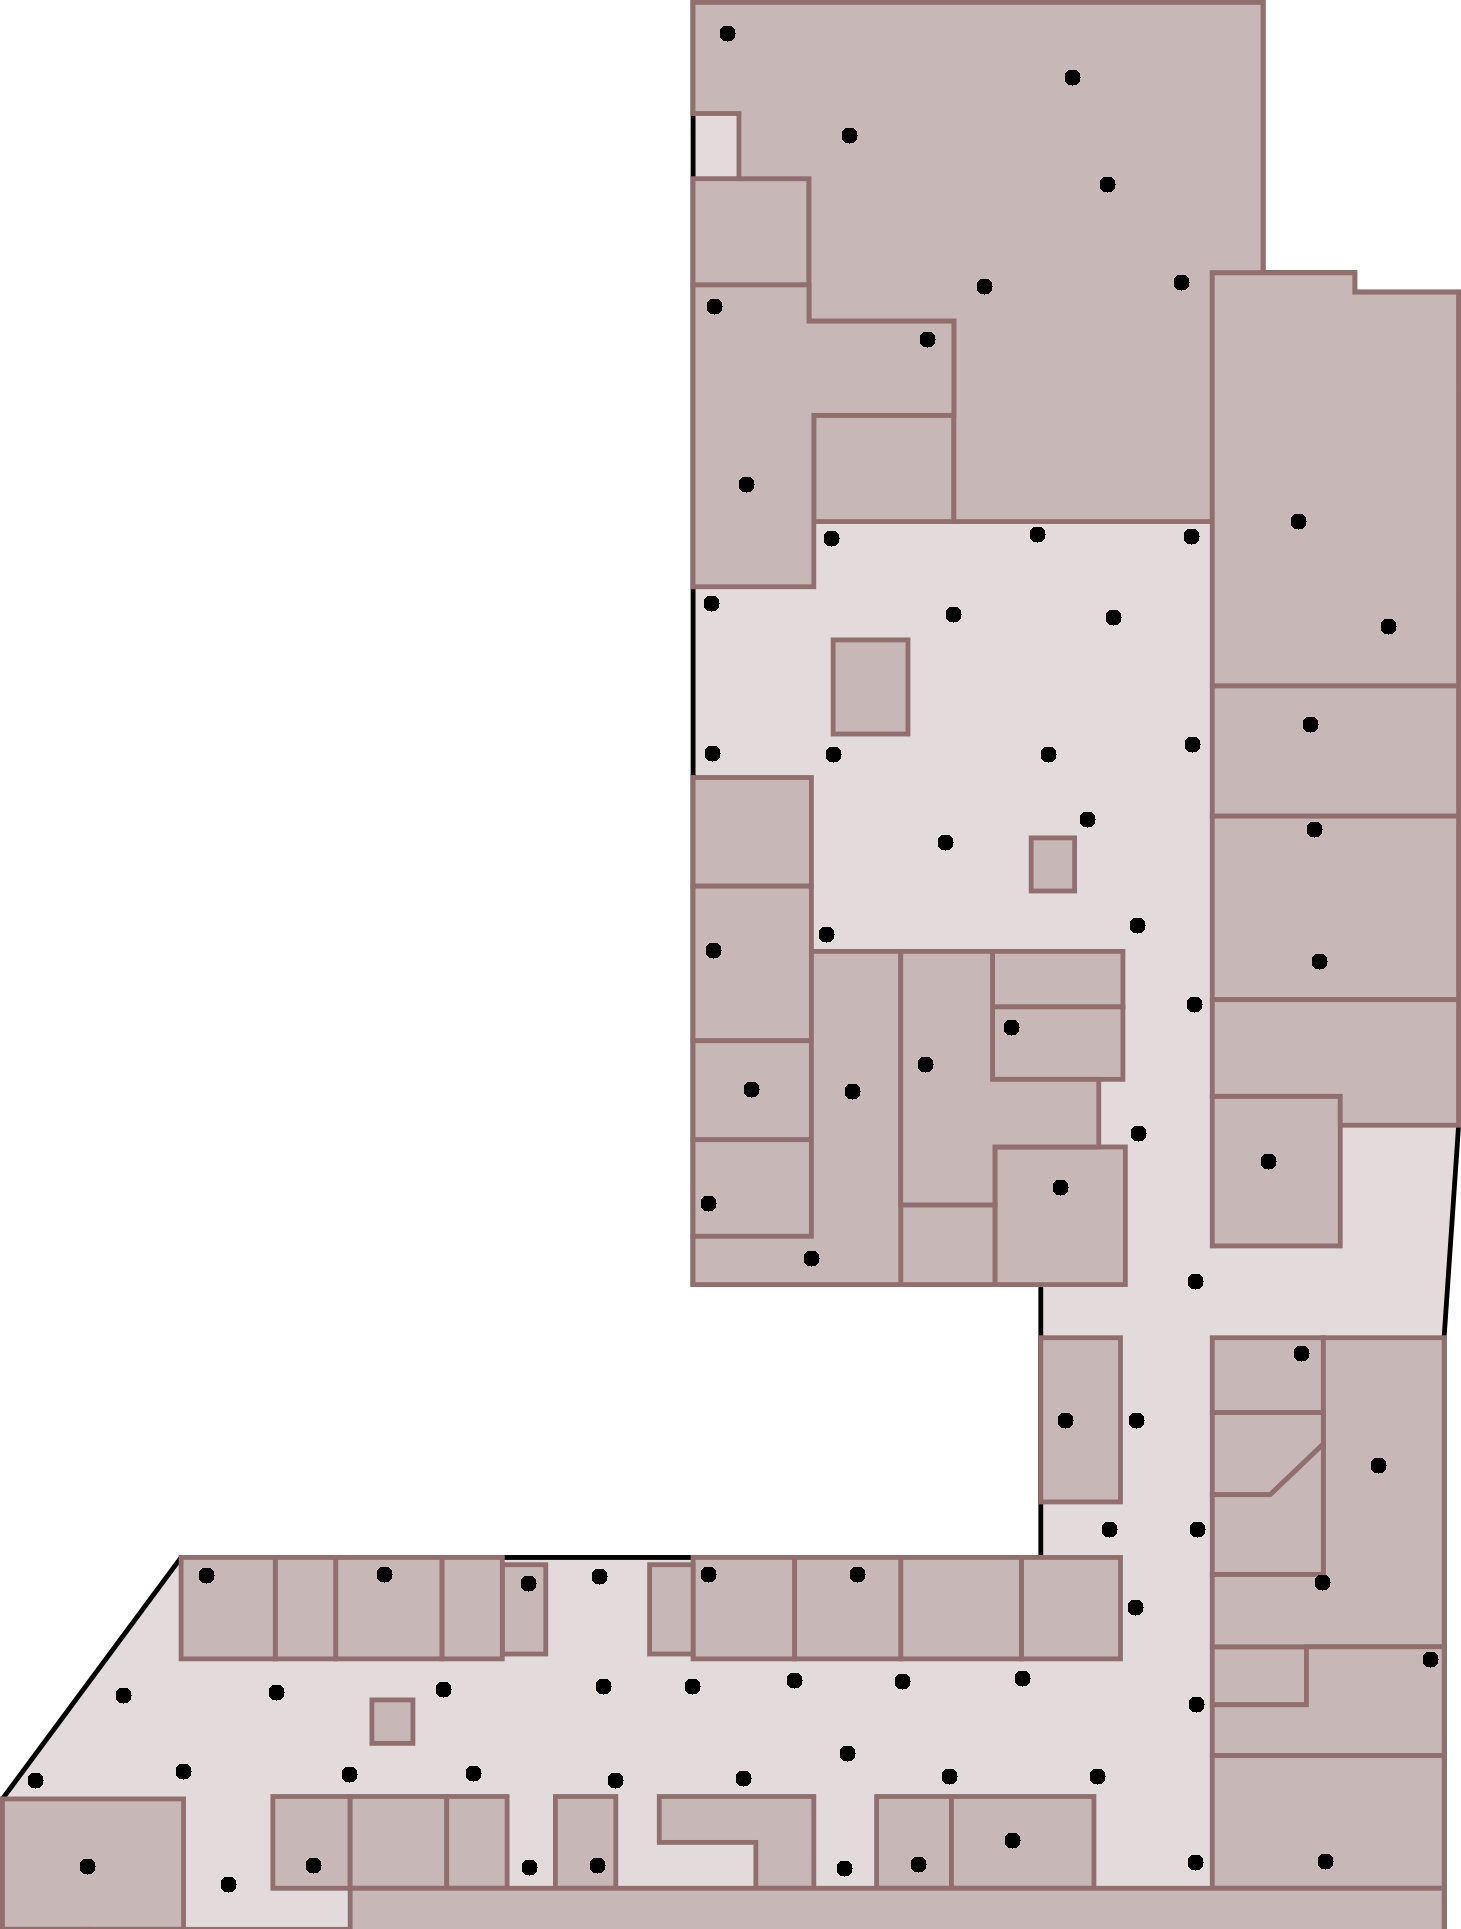
\includegraphics[width=7cm]{imatges/planol_log.png}
\caption{Punts on s'ha dut a terme la presa de dades.}
\label{fig:planol_log}
\end{center}
\end{figure}


Tenint en compte com pot afectar la presència d'usuaris en la potència de senyal rebut, es va considerar que la presa de dades s'havia de dur a terme en els moments de menys presència en el centre. L'horari comercial comença a les 10 del matí, però la presència d'oficines en l'interior de l'edifici fa que els passadissos siguin accessibles des de les 8 del matí. Tenint això en compte, tot el procés de presa de mesures per construir el mapa de ràdio va tenir lloc durant dos dies únicament entre les 8 i les 9 del matí. En quant a la presa de dades dins les tendes, s'ha de tenir en compte que, depenent del dia, i des del primer moment d'obertura, la presència de clients és un factor crític en la tasca de realitzar el mapa de ràdio. En el nostre cas, la presa de dades es va dur a terme des del moment d'obertura dels locals comercials i només fins que l'absència de clients permetés una presa de dades convenient (normalment entre 30 i 60 minuts), fet que va allargar la tasca durant quatre dies, El nombre de mesures dins tendes varia segons l'àrea ocupada per cada una.

També s'ha de tenir en compte quins valors fixar, tenint en compte que en l'AirPlace Logger es poden definir la quantitat de mostres a prendre en cada punt a localitzar i l'interval de temps entre mostres. Com que el senyal rebut des d'un punt d'accés WiFi fluctua notablement i la potència rebuda mesurada varia al llarg del temps, s'ha cregut convenient enregistrar el màxim nombre de mostres possibles, en aquest cas 30. Com que ens interessa enregistrar el major nombre de variacions per tal d'obtenir una mitja més acurada, l'interval entre cada mostra s'ha fixat en 1 segon, ja que mig segon entre mostres podria resultar en una mostra poc fluctuant, i dos segons hauria allargat massa el temps de presa de dades. A la figura \ref{fig:fluctuacio} es mostra la variació de la potència del senyal rebut en un punt al llarg de les 30 mostres. Com s'observa, en un punt la intensitat rebuda pot variar fins a 15 dbm, el que influeix en la poca precisió dels sistemes de localització per WiFi.

\begin{figure}[ht]
\begin{center}
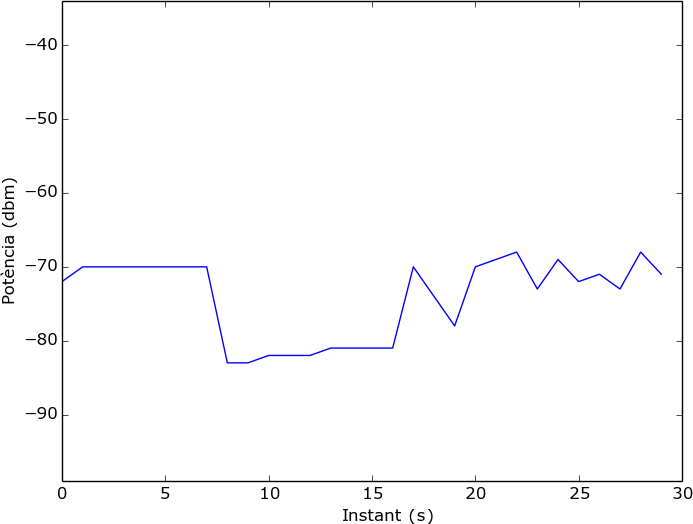
\includegraphics[width=7cm]{imatges/fluctuacio.png}
\caption{Variació de la potència del senyal rebut per la MAC f8:63:94:9c:2e:db al punt P74.}
\label{fig:fluctuacio}
\end{center}
\end{figure}

A més, es va dur una segona presa de dades per tal de calcular, utilitzant el AirPlace Radio Map Server, els valors més adients pels algorismes de aproximació de la localització. Aquesta presa de dades va seguir els mateixos criteris que els tinguts en compte a l'hora d'elaborar el mapa de ràdio. En aquest cas, es varen prendre mesures en 84 punts diferents, amb una distància mínima mitjana entre localitzacions de 7,51 m., i una distància mínma màxima de 11,85 m. La figura \ref{fig:planol_test} mostra la representació d'aquestes mostres damunt el pla.

\begin{figure}[ht]
\begin{center}
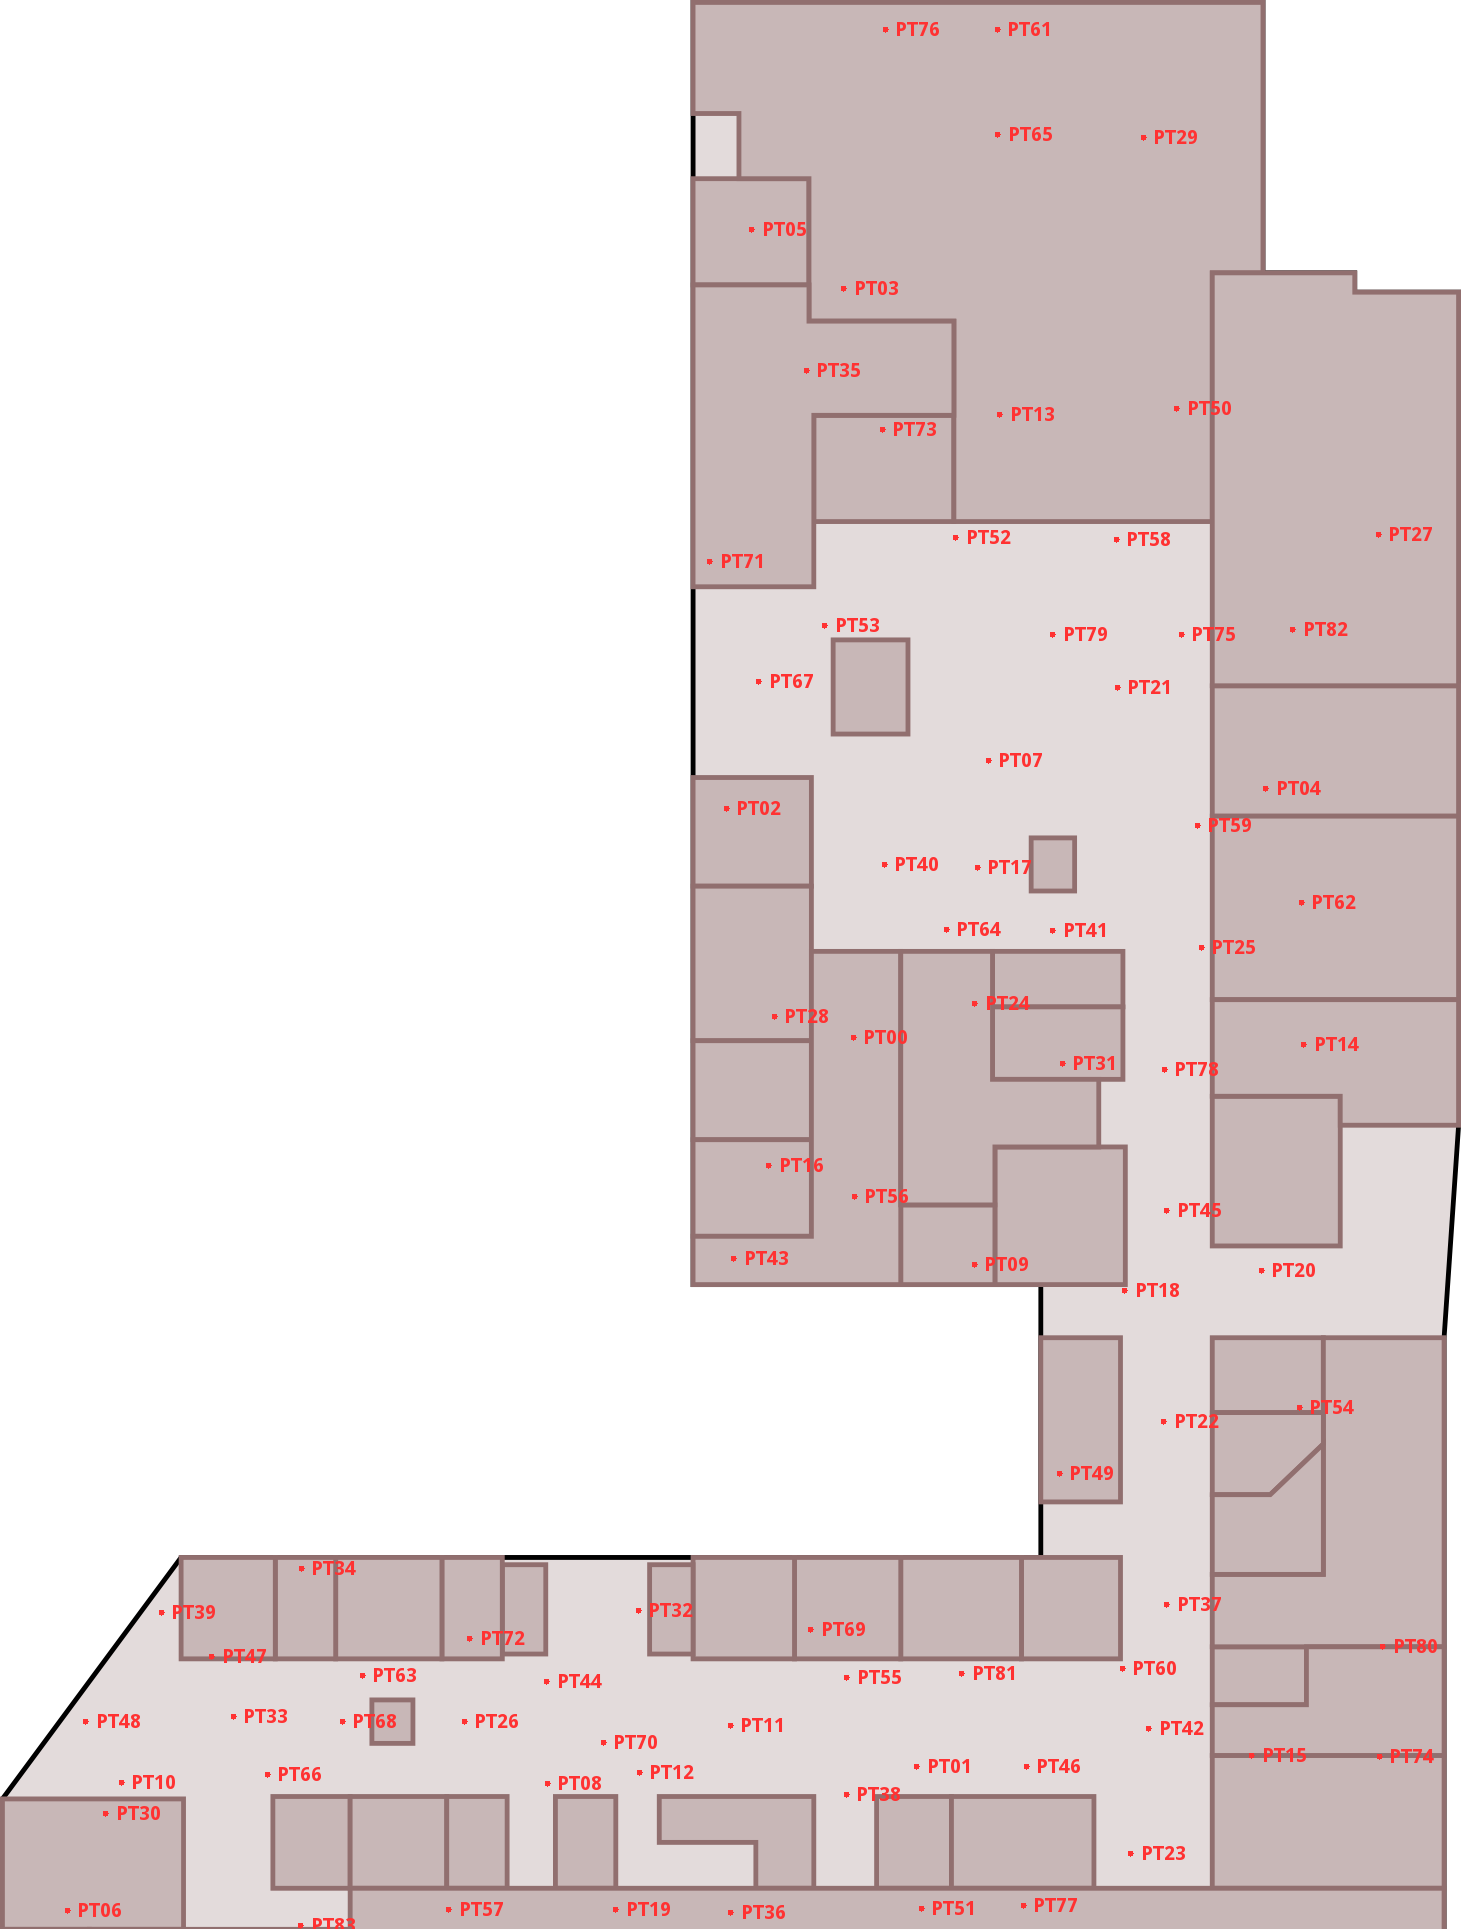
\includegraphics[width=7cm]{imatges/planol_test.png}
\caption{Punts on s'ha dut a terme la presa de dades de test.}
\label{fig:planol_test}
\end{center}
\end{figure}
